\documentclass[12pt]{article}
\usepackage[left=1cm, right=1cm, top=2cm,bottom=1.5cm]{geometry} 

\usepackage[parfill]{parskip}
\usepackage[utf8]{inputenc}
\usepackage[T2A]{fontenc}
\usepackage[russian]{babel}
\usepackage{enumitem}
\usepackage[normalem]{ulem}
\usepackage{amsfonts, amsmath, amsthm, amssymb, mathtools}
\usepackage{tabularx}
\usepackage{hhline}

\usepackage{accents}
\usepackage{fancyhdr}
\pagestyle{fancy}
\renewcommand{\headrulewidth}{1.5pt}
\renewcommand{\footrulewidth}{1pt}

\usepackage{graphicx}
\usepackage[figurename=Рис.]{caption}
\usepackage{subcaption}
\usepackage{float}

%%Наименование папки откуда забирать изображения
\graphicspath{ {./images/} }

%%Изменение формата для ввода доказательства
\renewcommand{\proofname}{$\square$  \nopunct}
\renewcommand\qedsymbol{$\blacksquare$}

%%Изменение отступа на таблицах
\addto\captionsrussian{%
	\renewcommand{\proofname}{$\square$ \nopunct}%
}
%% Римские цифры
\newcommand{\RN}[1]{%
	\textup{\uppercase\expandafter{\romannumeral#1}}%
}

%% Для удобства записи
\newcommand{\MR}{\mathbb{R}}
\newcommand{\MQ}{\mathbb{Q}}
\newcommand{\MN}{\mathbb{N}}
\newcommand{\MTB}{\mathbb{T}}
\newcommand{\MI}{\mathrm{I}}
\newcommand{\MJ}{\mathrm{J}}
\newcommand{\MH}{\mathrm{H}}
\newcommand{\MT}{\mathrm{T}}
\newcommand{\MU}{\mathcal{U}}
\newcommand{\MV}{\mathcal{V}}
\newcommand{\MW}{\mathcal{W}}
\newcommand{\VN}{\varnothing}
\newcommand{\VE}{\varepsilon}

\theoremstyle{definition}
\newtheorem{defn}{Опр:}
\newtheorem{rem}{Rm:}
\newtheorem{prop}{Утв.}
\newtheorem{exrc}{Упр.}
\newtheorem{lemma}{Лемма}
\newtheorem{theorem}{Теорема}
\newtheorem{corollary}{Следствие}

\newenvironment{cusdefn}[1]
{\renewcommand\thedefn{#1}\defn}
{\enddefn}

\DeclareRobustCommand{\divby}{%
	\mathrel{\text{\vbox{\baselineskip.65ex\lineskiplimit0pt\hbox{.}\hbox{.}\hbox{.}}}}%
}
%Короткий минус
\DeclareMathSymbol{\SMN}{\mathbin}{AMSa}{"39}
%Длинная шапка
\newcommand{\overbar}[1]{\mkern 1.5mu\overline{\mkern-1.5mu#1\mkern-1.5mu}\mkern 1.5mu}
%Функция знака
\DeclareMathOperator{\sgn}{sgn}

%Функция ранга
\DeclareMathOperator{\rk}{\text{rk}}

%Обозначение константы
\DeclareMathOperator{\const}{\text{const}}

%Интеграл в большом формате
\DeclareMathOperator{\dint}{\displaystyle\int}
\newcommand{\ddint}[2]{\displaystyle\int\limits_{#1}^{#2}}

\newcommand{\smallerrel}[1]{\mathrel{\mathpalette\smallerrelaux{#1}}}
\newcommand{\smallerrelaux}[2]{\raisebox{.1ex}{\scalebox{.75}{$#1#2$}}}

\newcommand{\smallin}{\smallerrel{\in}}
\newcommand{\smallnotin}{\smallerrel{\notin}}

\newcommand*{\medcap}{\mathbin{\scalebox{1.25}{\ensuremath{\cap}}}}%
\newcommand*{\medcup}{\mathbin{\scalebox{1.25}{\ensuremath{\cup}}}}%

\makeatletter
\newcommand{\vast}{\bBigg@{3.5}}
\newcommand{\Vast}{\bBigg@{5}}
\makeatother

%Скалярное произведение
\DeclarePairedDelimiterX{\inner}[2]{\langle}{\rangle}{#1, #2}

%Подпись символов снизу
\newcommand{\ubar}[1]{\underaccent{\bar}{#1}}

\begin{document}
\lhead{Математический анализ - \RN{2}}
\chead{Шапошников С.В.}
\rhead{Лекция - 22}
\section*{Свойства интеграла Римана}
\begin{theorem}
	Пусть $f_n$ интегрируемы по Риману на отрезке $[a,b]$ и $f_n \rightrightarrows f$ на $[a,b]$. Тогда $f$ интегрируема по Риману на $[a,b]$ и верно следующее:
	$$
		\ddint{a}{b}f(x)dx = \lim\limits_{n \to \infty} \ddint{a}{b}f_n(x)dx
	$$
\end{theorem}
\begin{proof}\hfill\\
	$1)$ Докажем, что последовательность чисел $\ddint{a}{b}f_n(x)dx$ сходится. Рассмотрим критерий Коши и воспользуемся линейностью интеграла Римана:
	$$
		\left| \ddint{a}{b}f_n(x)dx - \ddint{a}{b}f_m(x)dx \right| = \left| \ddint{a}{b}\big(f_m(x) - f_n(x)\big)dx \right|
	$$
	Мы можем записать следующие неравенства:
	$$
		m = -\sup\limits_x{|f_n(x) - f_m(x)|} \leq f_n(x) - f_m(x) \leq \sup\limits_x{|f_n(x) - f_m(x)|} = M \
	$$
	и воспользоваться теоремой о среднем:
	$$
		\ddint{a}{b}\big(f_m(x) - f_n(x)\big)dx = \mu_{n,m}{\cdot}(b-a), \, m \leq \mu_{n,m} \leq M	
	$$
	где $\mu_{n,m} \in [m,M]$ и как следствие $|\mu_{n,m}| \leq \sup\limits_x{|f_n(x) - f_m(x)|}$. Тогда получим:
	$$
		\left| \ddint{a}{b}\big(f_m(x) - f_n(x)\big)dx \right| = \left|  \mu_{n,m}{\cdot}(b-a)  \right| \leq \sup\limits_x{|f_n(x) - f_m(x)|}{\cdot}(b-a) \xrightarrow[n,m\to \infty]{} 0
	$$
	где последнее верно по равномерной сходимости $f_n \rightrightarrows f$ (используя критерий Коши). Следовательно последовательность интегралов $\MI_n = \ddint{a}{b}f_n(x)dx$ фундаментальна и существует её предел $\MI = \lim\limits_{n\to \infty} \MI_n$.
	
	$2)$ Зафиксируем отмеченное разбиение $(\MTB,\xi)$ отрезка $[a,b]$ и воспользуемся правилом $3\VE$:
	$$
		|\MI - \sigma(f,\MTB,\xi)| \leq |\MI - \MI_n| + |\MI_n - \sigma(f_n,\MTB,\xi)| + |\sigma(f_n,\MTB,\xi) - \sigma(f,\MTB,\xi)| 
	$$
	Заметим, что:
	$$
		|\sigma(f_n,\MTB,\xi) - \sigma(f,\MTB,\xi)| = \left| \displaystyle \sum\limits_k \big(f_n(\xi_k) - f(\xi_k)\big){\cdot}|\Delta_k| \right| \leq \displaystyle \sum\limits_k \big|f_n(\xi_k) - f(\xi_k)\big|{\cdot}|\Delta_k|
	$$
	Поскольку $f_n$ стремится к $f$ равномерно, то $\forall k, \, \big|f_n(\xi_k) - f(\xi_k)\big| \leq \sup\limits_{x \in [a,b]}\big|f_n(x) - f(x)\big|$ и тогда верно:
	$$
		|\sigma(f_n,\MTB,\xi) - \sigma(f,\MTB,\xi)| \leq \displaystyle \sum\limits_k \underbrace{\big|f_n(\xi_k) - f(\xi_k)\big|}_{\leq \sup\limits_{x\in[a,b]}\big|f_n(x) - f(x)\big|}{\cdot}|\Delta_k| \leq (b-a){\cdot}\sup\limits_{x \in [a,b]}\big|f_n(x) - f(x)\big|
	$$
	Возьмем $\VE > 0$ и находим $n$ такое, что $|\MI - \MI_n| < \VE$ и $|\sigma(f_n,\MTB,\xi) - \sigma(f,\MTB,\xi)| < \VE$. Фиксируем $n$, поскольку по условию $f_n$ были интегрируемы, то находим $\delta > 0 \colon \lambda(\MTB) < \delta \Rightarrow |\MI_n - \sigma(f_n,\MTB,\xi)| < \VE$. Тогда:
	$$
		\forall \VE > 0, \, \exists \, \delta > 0 \colon \forall (\MTB, \xi), \, \lambda(\MTB) < \delta \Rightarrow |\MI - \sigma(f,\MTB,\xi)| < \VE + \VE + \VE = 3\VE
	$$
\end{proof}
\begin{rem}
	Данное доказательство напоминает доказательство сохранения непрерывности при равномерном пределе. Так получилось поскольку проблема в этих утверждения одна и та же: необходимо поменять два предела местами (предел в интеграле и предел $f_n$ в данном случае).
\end{rem}

\begin{corollary}
	Если $f$ непрерывна на отрезке $[a,b]$, то $f$ интегрируема по Риману на $[a,b]$.
\end{corollary}
\textbf{\uline{Идея}}: Необходимо придумать последовательность функций, которые будут равномерно приближать непрерывную функцию $f$. Будем использовать ступенчатые функции:
\begin{figure}[H]
	\centering
	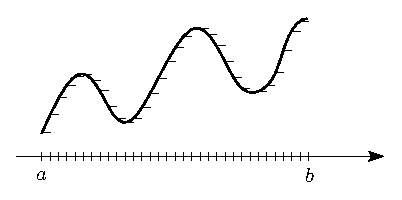
\includegraphics[width=0.4\textwidth]{22_1.eps}
	\caption{Приближение непрерывной функции ступенчатыми.}
	\label{22_1}
\end{figure}
разделим отрезок $[a,b]$ на части и на каждой заменим функцию $f$ каким-нибудь её значением $\Rightarrow$ получаем ступенчатую функцию. Разбивая всё мельче отрезок $[a,b]$, получим последовательность ступенчатых функций равномерно сходящихся к $f$.
\begin{proof}
	Пусть $\Delta_k^n = [x_{k-1}^n, x_k^n), \, \forall k = \overline{1,n-1}, \, \Delta_n^n = [x_{n-1}^n,b]$, где $x_k^n = a + \tfrac{k(b-a)}{n}$. Определим  $f_n(x)$:
	$$
		f_n(x) = \displaystyle \sum\limits_{k = 1}^n f(x_{k-1}^n){\cdot}\mathbb{I}_{\Delta_k^n}(x)
	$$
	Это последовательность интегрируемых функций, как линейная комбинация интегрируемых функций. Рассмотрим разность $|f_n(x) - f(x)|$:
	$$
		\forall x \in \Delta_k^n, \, |f_n(x) - f(x)| = |f(x_1^n){\cdot}0 + \dotsc + f(x_{k-1}^n){\cdot}1 + \dotsc + f(x_{n-1}^n){\cdot}0 - f(x)| = |f(x_{k-1}^n) - f(x)|
	$$
	Поскольку функция $f$ непрерывна на $[a,b] \Rightarrow$ по теореме Кантора функция $f$ равномерно непрерывна:
	$$
		\forall \VE > 0, \, \exists \, \delta > 0 \colon \forall x,y \in [a,b],\, |x - y| < \delta \Rightarrow |f(x) - f(y)| < \VE 
	$$
	Следовательно при каждом фиксированном $n$ и $k$ будет верно:
	$$
		\forall \VE > 0, \, \exists \, \delta > 0 \colon \forall x \in \Delta_k^n, \, |x - x_{k-1}^n| < \delta \Rightarrow |f(x_{k-1}^n) - f(x)| = |f_n(x) - f(x)| < \VE
	$$
	Длина каждого из отрезков разбиения $|\Delta_k^n| \leq |x_k^n - x_{k-1}^n| = \tfrac{b-a}{n}$ стремится к нулю с ростом $n$, тогда $\forall k$:
	$$
		\forall \delta > 0, \, \exists \, N \colon \forall n > N, \, |\Delta_k^n| < \delta
	$$
	Поскольку $\forall x \in \Delta_k^n$ верно $|x - x_{k-1}^n| < |\Delta_k^n|$, то $\forall k, \, \forall x \in \Delta_k^n$ мы получим:
	$$
		\forall \VE > 0, \, \exists \, N \colon \forall n > N, \, |f(x_{k-1}^n) - f(x)|  = |f_n(x) - f(x)| < \VE
	$$
	В силу того, что $[a,b] = \bigcup\limits_{k=1}^n\Delta_k^n$ это же будет верно для любой точки $x \in [a,b]$. Тогда по определению точной верхней грани:
	$$
		\forall \VE > 0, \, \exists \, N \colon \forall n > N, \, \sup\limits_{x \in [a,b]}|f_n(x) - f(x)| \leq \VE 
	$$
	Из чего следует, что $f_n \rightrightarrows f$. Применяем предыдущую теорему и получаем требуемое.
\end{proof}
\begin{exrc}
	Пусть $f$ кусочно-непрерывная функция на отрезке $[a,b]$, то есть: существует конечный набор точек $(a = c_0,\dotsc, c_m = b)$ таких, что на каждом интервале $(c_i, c_{i+1})$ функция $f$ непрерывна и верно:
	$$
		\forall i = \overline{0,m-1}, \, \exists \, f(c_i+) = \lim\limits_{x \to c_i +}f(x), \, \forall i = \overline{1, m}, \, \exists \, f(c_i \SMN) = \lim\limits_{x \to c_i -}f(x)
	$$ 
	или по-другому: функция разрывна, но у неё конечное число точек разрыва, каждая из которых это разрыв первого рода. Доказать, что кусочно-непрерывная функция $f$ интегрируема по Риману.
\end{exrc}
\begin{proof}
	Пусть $\forall i = \overline{1,m},\, \Delta_{i,k}^n = [x_{i,k-1}^n, x_{i,k}^n), \,  \forall k = \overline{2,n}$ и $\Delta_{i,1}^n = (x_{i,0}^n, x_{i,1}^n)$, где $x_{i,k}^n = c_{i-1} + \tfrac{k(c_i - c_{i-1})}{n}$. Определим функцию $f_n(x)$ следующим образом:
	$$
		f_n(x) = f_n^1(x) + \dotsc + f_n^m(x) + f(c_0){\cdot}\mathbb{I}_{c_0}(x) + \dotsc + f(c_m){\cdot}\mathbb{I}_{c_m}(x) 
	$$
	$$
		\forall i = \overline{1,m}, \, f_n^i(x) = \displaystyle \sum\limits_{k = 2}^n f(x_{i,k-1}^n){\cdot}\mathbb{I}_{\Delta_{i,k}^n}(x) + f(x_{i,0}^n\SMN){\cdot}\mathbb{I}_{\Delta_{i,1}^n}(x)
	$$
	Это последовательность интегрируемых функций, как линейная комбинация интегрируемых функций. Рассмотрим разность $|f_n(x) - f(x)|$:
	$$
		\forall x \in \Delta_{i,k}^n, \, k \neq 1, \, |f_n(x) - f(x)| = |f(x_{i,k-1}^n){\cdot}1 - f(x)| = |f(x_{i,k-1}^n) - f(x)|
	$$
	$$
		\forall x \in \Delta_{i,1}^n, \, |f_n(x) - f(x)| = |f(x_{i,1}^n\SMN){\cdot}1 - f(x)| = |f(x_{i,0}^n\SMN) - f(x)|
	$$
	$$
		\forall i = \overline{0,m}, \, x = c_i \Rightarrow |f_n(x) - f(x)| = |0 + \dotsc + 0 + f(c_i){\cdot}1 + 0 + \dotsc + 0 - f(c_i)| = |f(c_i) - f(c_i)| = 0 
	$$
	Рассмотрим следующую функцию на отрезке $[c_{i-1},c_i], \, \forall i = \overline{1,m}$:
	$$
		\widetilde{f}_i(x) = 
		\left\{
			\begin{array}{ll}
				f(x), & x \in (c_{i-1},c_i) \\
				f(c_{i-1}+), & x = c_{i-1} \\
				f(c_i \SMN), &  x = c_i  
			\end{array}
		\right.
	$$
	По определению она будет непрерывна на отрезке $[c_{i-1},c_i] \Rightarrow$ по теореме Кантора функция $\widetilde{f}_i(x)$ будет равномерно непрерывна на этом отрезке. Тогда:
	$$
		\forall \VE > 0, \, \exists \, \delta > 0 \colon \forall x,y \in [c_{i-1},c_i],\, |x - y| < \delta \Rightarrow \left|\widetilde{f}_i(x) - \widetilde{f}_i(y)\right| < \VE 
	$$
	Следовательно это же будет справедливо и $\forall x \in \Delta_{i,k}^n \subset (c_{i-1},c_i)$. Таким образом, при каждом фиксированном $n, \, i$ и $k \neq 1$ будет верно:
	$$
		\forall \VE > 0, \, \exists \, \delta > 0 \colon \forall k \neq 1, \, \forall x \in \Delta_{i,k}^n, \, |x - x_{i,k-1}^n| < \delta \Rightarrow |f(x_{i,k-1}^n) - f(x)| = |f_n(x) - f(x)| < \VE
	$$
	Также, по определению одностороннего предела, при каждом фиксированном $n$ и $i$:
	$$
		\forall \VE > 0, \, \exists \, \delta > 0 \colon \forall x \in \Delta_{i,1}^n, \, 0 < x - x_{i,0}^n < \delta \Rightarrow |f(x_{i,0}^n\SMN) - f(x)| = |f_n(x) - f(x)| < \VE
	$$
	Длина каждого из отрезков разбиения $|\Delta_{i,k}^n| < |x_{i,k}^n - x_{i,k-1}^n| = \tfrac{c_i - c_{i-1}}{n}, \, \forall i = \overline{1,m}$ стремится к нулю с ростом $n$, тогда $\forall k,i$:
	$$
		\forall \delta > 0, \, \exists \, N \colon \forall n > N, \, |\Delta_{i,k}^n| < \delta
	$$
	Поскольку $\forall x \in \Delta_{i,k}^n$ верно $|x - x_{i,k-1}^n| < |\Delta_{i,k}^n|$, то $\forall k,i, \, \forall x \in \Delta_{i,k}^n$ мы получим, что $\forall \VE > 0, \, \exists \, N \colon \forall n > N$:
	$$
		k \neq 1,  \, |f(x_{i,k-1}^n) - f(x)|  = |f_n(x) - f(x)| < \VE
	$$
	$$
		k = 1,\, |f(x_{i,0}^n\SMN) - f(x)|  = |f_n(x) - f(x)| < \VE
	$$
	В силу того, что $[a,b] = \bigcup\limits_{k=1}^n\bigcup\limits_{i=1}^m\Delta_{i,k}^n \cup \bigcup\limits_{i=0}^m c_i$ это же будет верно для любой точки $x \in [a,b]$. Тогда по определению точной верхней грани:
	$$
		\forall \VE > 0, \, \exists \, N \colon \forall n > N, \, \sup\limits_{x \in [a,b]}|f_n(x) - f(x)| \leq \VE 
	$$
	Из чего следует, что $f_n \rightrightarrows f$. Применяем предыдущую теорему и получаем требуемое.
\end{proof}

\begin{corollary}
	Если $f$ монотонна на $[a,b]$, то $f$ интегрируема по Риману на $[a,b]$.
\end{corollary}
\begin{rem}
	Заметим, что функция $f$ везде определена на отрезке $[a,b]$. Например, функция $f(x) = \tfrac{1}{x}$ на отрезке $[0,1]$ не подойдет под условия теоремы.
\end{rem}
\begin{rem}	
	Это утверждение нельзя вывести из предыдущего упражнения, поскольку у монотонной функции может быть бесконечно много (не более, чем счётно) точек разрыва. Тем не менее, все эти точки - это точки разрыва первого рода.
\end{rem}
Построить доказательство по аналогии с предыдущими следствиями невозможно из-за того, что точки разрыва всюду плотные. Поэтому будем строить разбиение не отрезка $[a,b]$, а образа этого отрезка.
\begin{proof}
	Без потери общности, пусть $f$ не убывает.
	\begin{figure}[H]
		\centering
		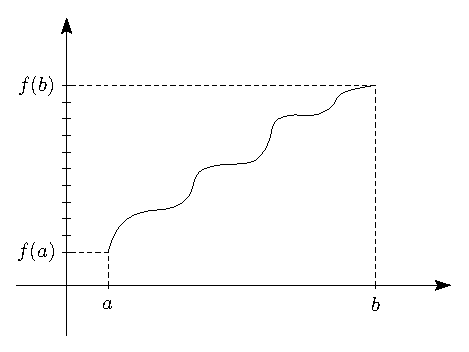
\includegraphics[width=0.4\textwidth]{22_2.eps}
		\caption{Монотонная функция $f$ и разбиение $[f(a),f(b)]$.}
		\label{22_2}
	\end{figure}
	\begin{enumerate}[label={\arabic*)}]
		\item Если $f(a) = f(b) \Rightarrow f = \const \Rightarrow$ утверждение доказано;
		\item Пусть $f(a) < f(b)$, будем строить последовательность $f_n$, которая приближает функцию $f$ равномерно. Тогда возьмем разбиение отрезка $[f(a),f(b)]$: 
		$$
			\forall k = \overline{1,n-1}, \, J_k^n = [y_{k-1}^n,y_k^n), \, J_n^n = [y_{n-1}^n, y_n^n], \,  y_k^n = f(a) + \dfrac{f(b) - f(a)}{n}{\cdot}k
		$$
		где $J_k$ попарно не пересекаются $\forall k = \overline{1,n}$. Рассмотрим прообраз каждого из этих промежутков:
		$$
			\Delta_k^n = f^{-1}(J_k^n) = \{x \in [a,b] \colon y_{k-1}^n \leq f(x) < y_k^n\}, \, k = \overline{1,n-1}
		$$
		$$
			\Delta_n^n = f^{-1}(J_n^n) = \{x \in [a,b] \colon y_{n-1}^n \leq f(x) \leq y_n^n\}
		$$
		В общем случае, прообразом может быть сложное множество, но у монотонных функций верно следующее:
		\begin{enumerate}[label={(\arabic*)}]
			\item $\Delta_k^n$ - промежуток;
			\begin{proof}
				Пусть $x_1 < x_2 < x_3, \, x_1, x_3 \in \Delta_k^n$. Поскольку $f(x)$ не убывает, то $y_{k-1}^n \leq f(x_1) \leq f(x_2)$, с другой стороны $f(x_2) \leq f(x_3) < y_k^n \Rightarrow x_2 \in \Delta_k^n \Rightarrow \Delta_k^n$ - промежуток.
			\end{proof}
			Заметим, что промежуток может состоять из одной точки, быть интервалом, отрезком или полуинтервалом;
			\item $\Delta_k^n \cap \Delta_l^n = \VN, \, \forall k \neq l$, то есть промежутки попарно не пересекаются;
			\begin{proof}
				Пусть $\Delta_k^n \cap \Delta_l^n \neq \VN$, тогда $\exists \, x \in \Delta_k^n \cap \Delta\colon y_{k-1}^n \leq f(x) < y_k^n \wedge y_{l-1}^n \leq f(x) < y_l^n$, откуда следует что $[y_{k-1}^n, y_k^n) \cap [y_{l-1}^n, y_l^n) \neq \VN \Rightarrow$ противоречие.
			\end{proof}
			\item $\bigcup\limits_k \Delta_k^n = [a,b]$;
			\begin{proof}
				Поскольку мы взяли прообразы всего, что есть в области значений $[f(a),f(b)]$, то мы получили весь отрезок $[a,b]$ в силу того, что $f$ определена на всем $[a,b]$.
			\end{proof}
		\end{enumerate}
		Рассмотрим следующие функции $f_n(x)$ и их разность с исходной функцией $f(x)$:
		$$
			f_n(x) = \displaystyle \sum\limits_{k = 1}^{n}y_{k-1}^n{\cdot}\mathbb{I}_{\Delta_k^n}(x) \Rightarrow \forall k, \, \forall x \in \Delta_k^n, \, |f_n(x) - f(x)| = |f(x) - y_{k-1}^n| \leq y_k^n - y_{k-1}^n = \dfrac{f(b) - f(a)}{n}
		$$
		\begin{figure}[H]
			\centering
			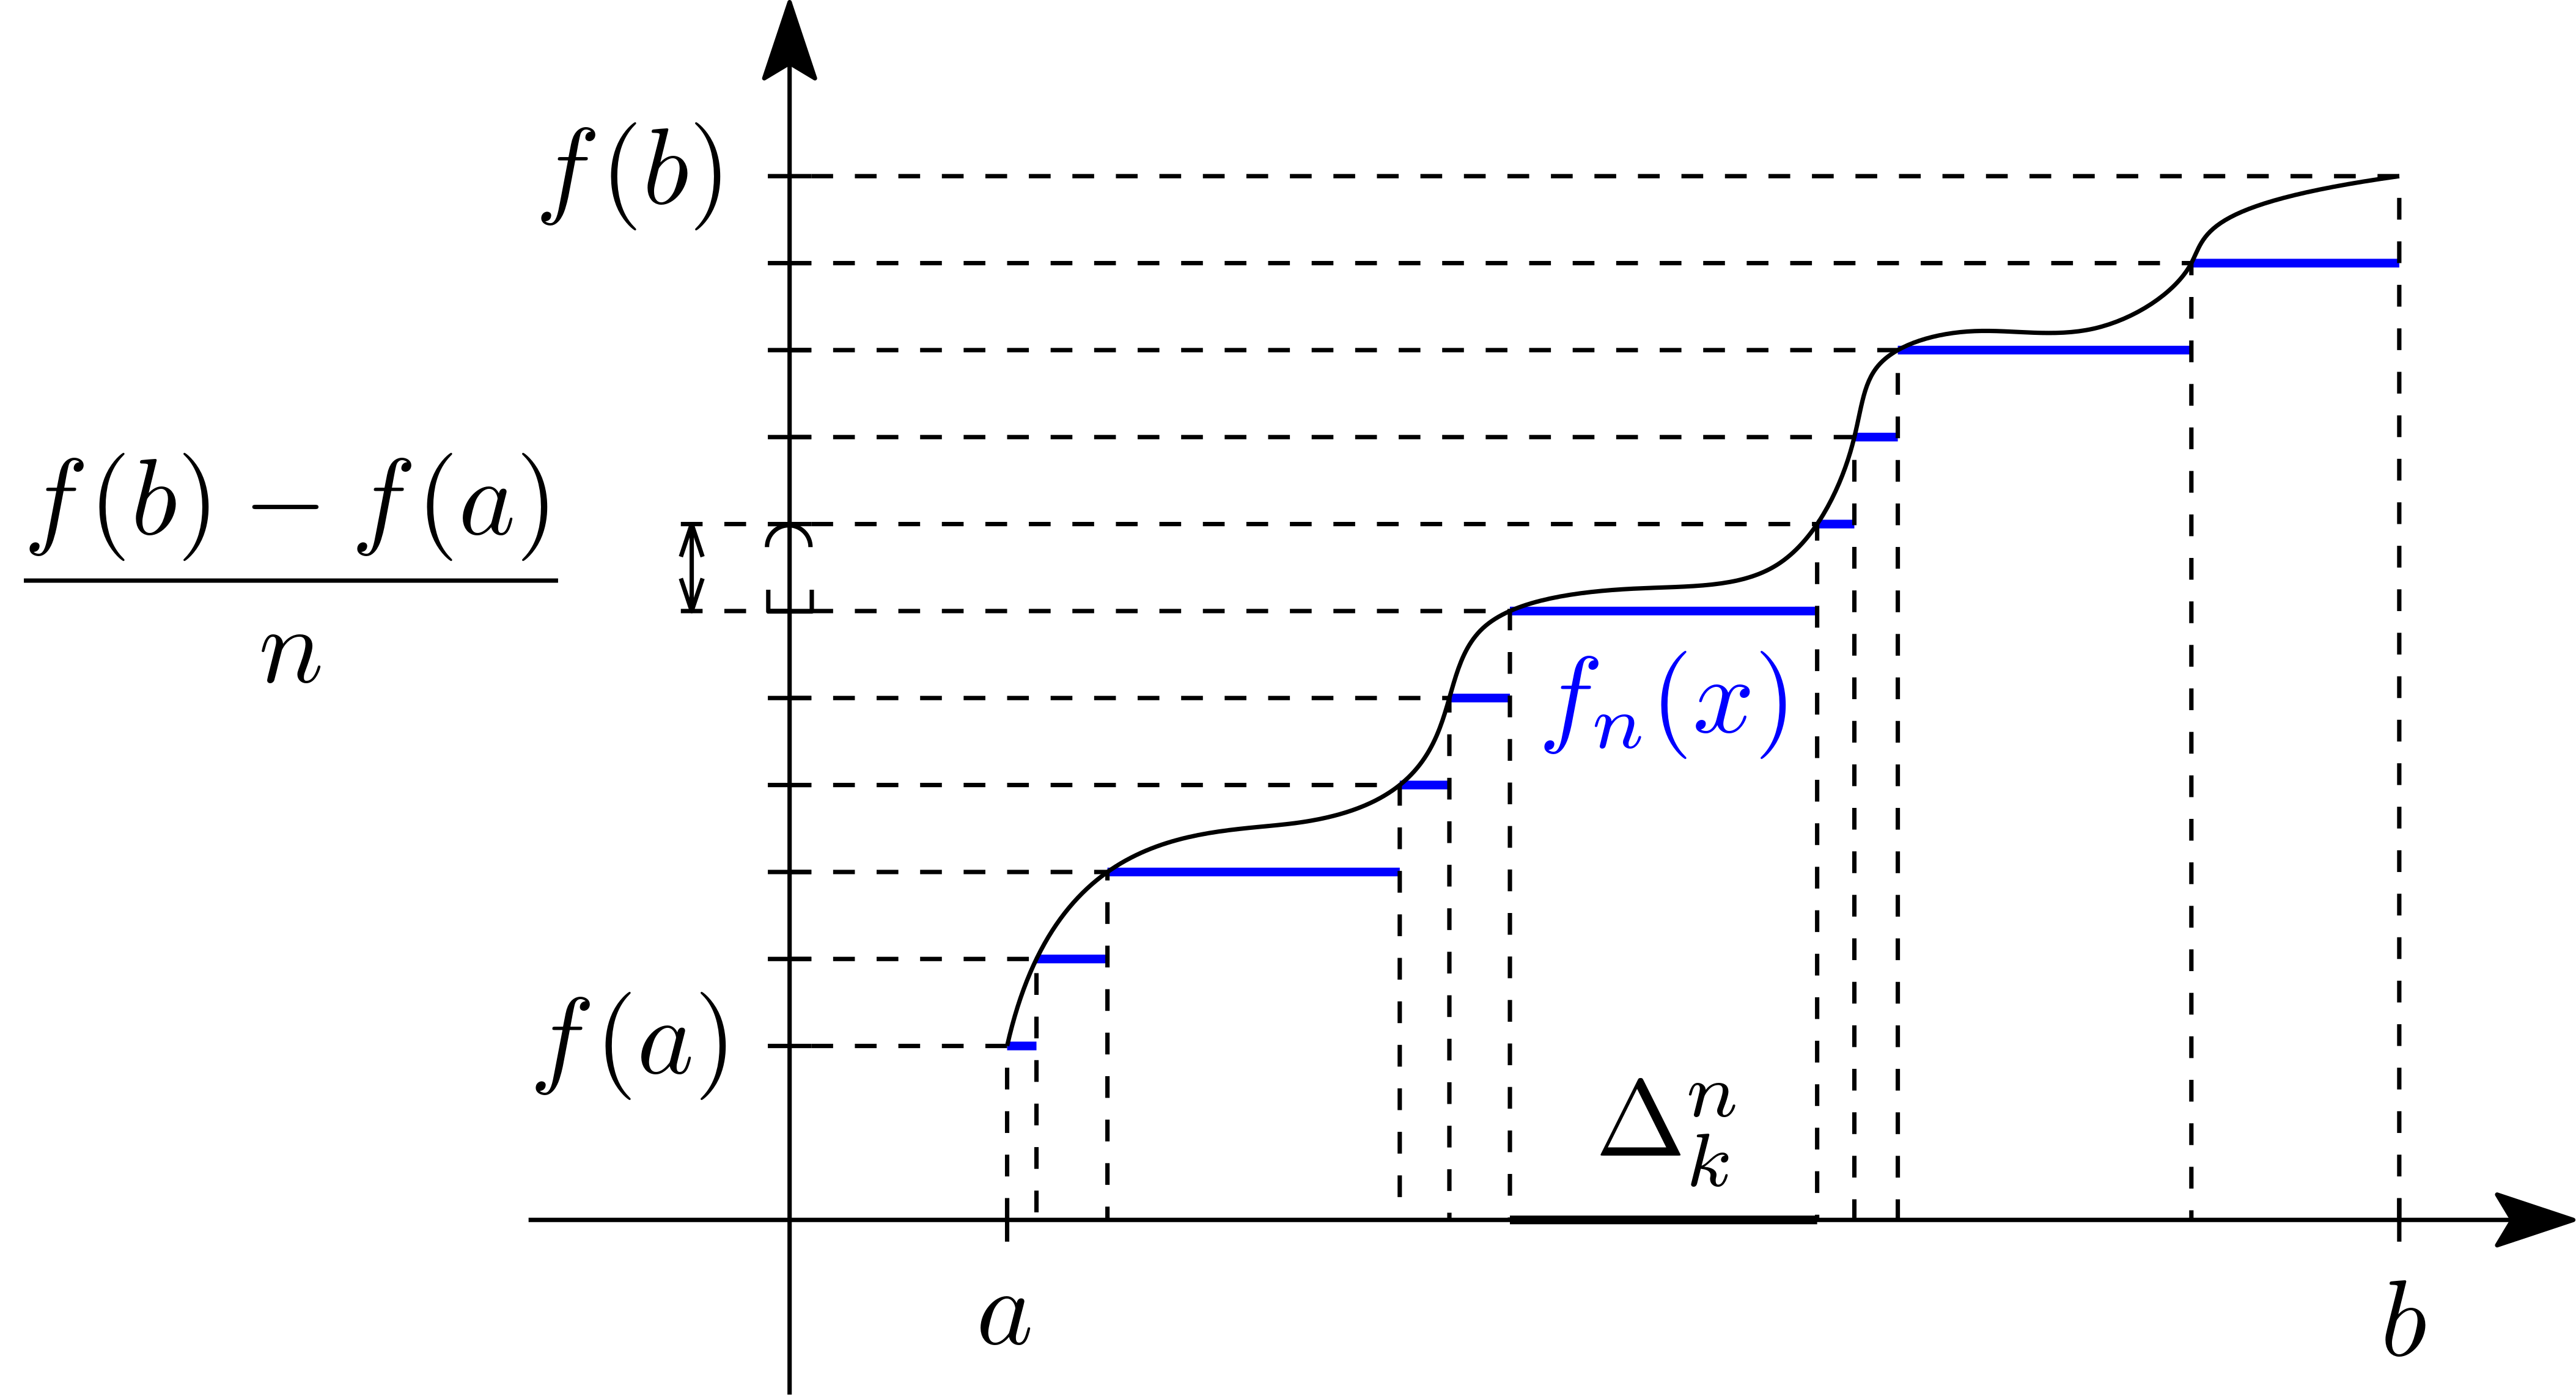
\includegraphics[width=0.55\textwidth]{22_3.png}
			\caption{Построение промежутков $\Delta_k^n$ и функций $f_n$.}
			\label{22_3}
		\end{figure}
		Таким образом, $f_n \rightrightarrows f$. Сами функции $f_n(x)$ - интегрируемые функции. Применяем предыдущую теорему и получаем требуемое.
	\end{enumerate}
\end{proof}

\begin{rem}
	Монотонность в доказательстве использовалась при построении множеств $\Delta_k^n$.
\end{rem}
\begin{rem}
	Из данного следствия мы знаем, что: 
	$$
		\ddint{a}{b}f(x)dx = \lim\limits_{n \to \infty}\displaystyle \sum\limits_{k = 1}^n \ddint{a}{b}f_n(x)dx=  \lim\limits_{n \to \infty}\displaystyle \sum\limits_{k = 1}^ny_{k-1}^n{\cdot}|\Delta_k^n|
	$$
	Если то же самое проделать не с монотонной функцией, а с любой ограниченной, то получим определение интеграла Лебега. Но возникает трудность в том, что $\Delta_k^n$ уже не обязательно будет промежутком и не ясно, что такое длина $\Delta_k^n$.
\end{rem}
Таким образом, мы получили достаточно широкий класс интегрируемых по Риману функций, которые можно приблизить ступенчатой функцией (непрерывные, кусочно-непрерывные, монотонные). Достаточно сложно придумать пример интегрируемое по Риману функции, которую нельзя приблизить ступенчатой.

$3)$ \textbf{(\uline{Аддитивность})}: Пусть $f$ интегрируема по Риману на отрезке $[a,b]$, отрезке $[a,c]$ и на отрезке $[c,b]$, где $a < c < b$, тогда:
$$
	\ddint{a}{b}f(x)dx = \ddint{a}{c}f(x)dx + \ddint{c}{b}f(x)dx
$$
\begin{rem}
	В данной формулировке есть избыточные условия, поскольку далее мы узнаем, что если функция интегрируема на отрезке, то она интегрируема на любом подотрезке и наоборот, если есть интегрируемость на $[a,c]$ и $[c,b]$, то есть интегрируемость на $[a,b]$.
\end{rem}
\begin{proof}
	Если интеграл существует, то его можно получить как предел по любой последовательности разбиений масштаб которой стремится к нулю. Возьмем последовательности разбиений: 
	$$
		\MTB_{[a,c]}^n \colon n\to \infty \Rightarrow \lambda\left(\MTB_{[a,c]}^n\right)\to 0, \, \MTB_{[c,b]}^n \colon n\to \infty \Rightarrow \lambda\left(\MTB_{[c,b]}^n\right)\to 0
	$$
	В частности, точка $c$ принадлежит обоим разбиениям. В каждом из разбиений $\MTB_{[a,c]}^n$ и $\MTB_{[c,b]}^n$ возьмем отмеченные точки $\xi^\prime$ и $\xi^{\prime\prime}$ соответственно. Возьмем разбиение $\MTB_{[a,b]}^n = \MTB_{[a,c]}^n \cup \MTB_{[c,b]}^n$, тогда объединение отмеченных точек каждого из разбиений $\xi = (\xi^\prime, \xi^{\prime\prime})$ будет отмеченными точками для большого разбиения отрезка $[a,b]$. Заметим, что:
	$$
		\lambda\left(\MTB_{[a,c]}^n\right)\to 0 \wedge \lambda\left(\MTB_{[c,b]}^n\right)\to 0 \Rightarrow \lambda\left(\MTB_{[a,b]}^n\right)\to 0
	$$
	$$
		\sigma\left(f,\MTB_{[a,b]}^n, \xi\right) = \sigma\left(f,\MTB_{[a,c]}^n, \xi^\prime\right) + \sigma\left(f,\MTB_{[c,b]}^n, \xi^{\prime\prime}\right)
	$$
	Тогда при $n \to \infty$ мы получим:
	$$
		\lim\limits_{n \to \infty} \sigma\left(f,\MTB_{[a,b]}^n, \xi\right) = \ddint{a}{b}f(x)dx = \lim\limits_{n \to \infty}\sigma\left(f,\MTB_{[a,c]}^n, \xi^\prime\right) + \lim\limits_{n \to \infty}\sigma\left(f,\MTB_{[c,b]}^n, \xi^{\prime\prime}\right) = \ddint{a}{c}f(x)dx + \ddint{c}{b}f(x)dx
	$$
\end{proof}
\begin{defn}
	Для дальнейшего удобства будем считать, что интеграл в точке равен нулю: 
	$$
		\ddint{a}{a}f(x)dx = 0
	$$
\end{defn}
\begin{defn}
	Пусть $a < b$, тогда будет верно равенство:
	$$
		\ddint{b}{a}f(x)dx = - \ddint{a}{b}f(x)dx
	$$
\end{defn}
\begin{rem}
	Эти равенства отлично согласуются с аддитивностью. Например, если во втором равенстве перенести интеграл и применить свойство аддитивности, то получим интеграл от $a$ до $a$, который будет равен нулю по первому равенству.
\end{rem}

$4)$ \textbf{(\uline{Формула Ньютона-Лейбница})}: Пусть $F$ дифференцируема на отрезке $[a,b]$ и $F^\prime$ интегрируема на отрезке $[a,b]$, тогда:
$$
	\ddint{a}{b}F^\prime(x)dx = F(b) - F(a)
$$
\begin{proof}
	Возьмем разбиение отрезка $[a,b]$ на $n$ частей $\MTB = \{a = x_0 < x_1 < \dotsc < x_n = b\}$. Тогда:
	$$
		F(b) - F(a) = \displaystyle \sum\limits_{k = 1}^{n}\big(F(x_{k}) - F(x_{k-1})\big) = \big(F(x_1) - F(a)\big) + \big(F(x_2) - F(x_1)\big) + \dotsc + \big(F(b) - F(x_{n-1})\big)
	$$
	Следовательно, по теореме Лагранжа будет верно:
	$$
		\displaystyle \sum\limits_{k = 1}^{n}\big(F(x_{k}) - F(x_{k-1})\big) = \displaystyle \sum\limits_{k = 1}^{n}F^\prime(c_k){\cdot}|\Delta_k|, \, \forall k = \overline{1,n}, \,  c_k \in (x_{k-1},x_k) \subset \Delta_k = [x_{k-1}, x_k]
	$$
	А это есть ничто иное, как Риманова сумма:
	$$
		\displaystyle \sum\limits_{k = 1}^{n}F^\prime(c_k){\cdot}|\Delta_k| = \sigma \left(F^\prime,\MTB,c \right), \, c = (c_1,\dotsc, c_n), \, \forall k, \, c_k \in \Delta_k 
	$$
	Таким образом, по определению интегрируемости на отрезке мы получим:
	$$
		\lim\limits_{\lambda(\MTB) \to 0}\big(F(b) - F(a)\big) = F(b) - F(a) =  \lim\limits_{\lambda(\MTB) \to 0}\sigma \left(F^\prime,\MTB,c \right) = \ddint{a}{b}F^\prime(x)dx
	$$
\end{proof}
В условиях формулы Ньютона-Лейбница, мы можем найти $F(b)$ используя интеграл Римана. Поскольку мы ищем интегралы с точностью до константы, предположим, что $F(a) = 0$, тогда:
$$
	F(x) = \ddint{a}{x}F^\prime(t)dt
$$
Таким образом, формула Ньютона-Лейбница отвечает на вопрос, как найти первообразную, производная которой интегрируема. Тем не менее, мы пока не можем ответить: есть ли первообразная у интегрируемой функции $f$.
\pagebreak
\section*{Интеграл с переменным верхним пределом}
Пусть $f$ - интегрируема на $[a,b]$. Существует ли у неё первообразная? В общем случае, ответ - нет.

\textbf{Пример}: Рассмотрим функцию $f(x) = \sgn(x) = \left\{
\begin{array}{rl}
	1, & x \in (0,1] \\
	0, & x = 0 \\
	1, & x \in [-1,0)
\end{array}\right.$ на отрезке $[-1,1]$.
\begin{figure}[H]
	\centering
	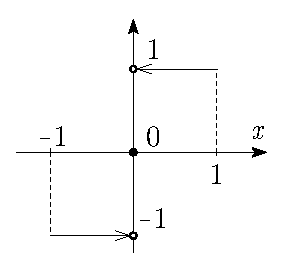
\includegraphics[width=0.25\textwidth]{22_4.eps}
	\caption{Функция $\sgn(x)$.}
	\label{22_4}
\end{figure}
Она интегрируема, но не имеет первообразной, поскольку не существует функции, производная которая была бы равна разрывной ступени. 

Таким образом, хотелось бы доказать, что для каких-то классов функций первообразная есть. Для этой цели будем использовать следующее определение.
\begin{defn}
	Пусть функция $f$ - интегрируема на $[a,b]$, тогда функция $F(x)$, заданная равенством:
	$$
		F(x) = \ddint{a}{x}f(t)dt
	$$
	называется \uwave{интегралом с переменным верхним пределом}.
\end{defn}

К примеру, для функции $f(x) = \sgn(x)$ мы получим следующий интеграл:
$$
	F(x) = \ddint{-1}{x}\sgn(t)dt = |x| - 1
$$
Эта функция не дифференцируема в нуле из-за того, что у $f(x)$ в этой точке разрыв.

\begin{theorem}
	Пусть $f$ непрерывна на отрезке $[a,b]$, тогда функция $F(x) = \ddint{a}{x}f(t)dt$ дифференцируема на $[a,b]$ и $F^\prime(x) = f(x), \, \forall x \in [a,b]$. Тем самым, у всякой непрерывной функции есть первообразная.
\end{theorem}
\begin{proof}
	Пусть $h > 0$, рассмотрим следующее отношение:
	$$
		\dfrac{F(x + h) - F(x)}{h} = \dfrac{1}{h}{\cdot}\!\!\left(\ddint{a}{x + h} f(t)dt - \ddint{a}{x}f(t)dt\right) = \dfrac{1}{h}\ddint{x}{x + h} f(t)dt 
	$$
	где последнее равенство верно в силу аддитивности. По теореме о среднем получим:
	$$
		\dfrac{1}{h}\ddint{x}{x + h} f(t)dt  = \dfrac{1}{h}{\cdot}f(c){\cdot}(x + h - x) = \dfrac{1}{h}{\cdot}f(c){\cdot}h = f(c), \, c \in [x, x + h]
	$$
	По непрерывности функции $f$ получаем следующее:
	$$
		\lim\limits_{h \to 0+} \dfrac{F(x + h) - F(x)}{h} = 	\lim\limits_{h \to 0+}f(c) = f(x)
	$$
	Пусть $h < 0$, по аналогии:
	$$
		\dfrac{F(x + h) - F(x)}{h} = \dfrac{1}{h}{\cdot}\!\!\left(\ddint{a}{x + h} f(t)dt - \ddint{a}{x}f(t)dt\right) = -\dfrac{1}{h}\ddint{x + h}{x} f(t)dt 
	$$
	где последнее равенство верно в силу аддитивности. По теореме о среднем получим:
	$$
		-\dfrac{1}{h}\ddint{x + h}{x} f(t)dt  = -\dfrac{1}{h}{\cdot}f(c){\cdot}(x - x - h) = \dfrac{1}{h}{\cdot}f(c){\cdot}h = f(c), \, c \in [x + h, x]
	$$
	По непрерывности функции $f$ получаем следующее:
	$$
		\lim\limits_{h \to 0-} \dfrac{F(x + h) - F(x)}{h} = 	\lim\limits_{h \to 0-}f(c) = f(x)
	$$
	Подводя итог, мы получим:
	$$
		\lim\limits_{h \to 0-} \dfrac{F(x + h) - F(x)}{h} = f(x) = \lim\limits_{h \to 0+} \dfrac{F(x + h) - F(x)}{h} = \lim\limits_{h \to 0} \dfrac{F(x + h) - F(x)}{h} = F^\prime(x)
	$$
	И таким образом будет верно, что $F^\prime(x) = f(x)$.
\end{proof}

\end{document}